
\documentclass[journal,12pt,twocolumn]{IEEEtran}
\usepackage{tkz-euclide} % loads TikZ and tkz-base
\usepackage{hyperref}
\usepackage{xcolor}
\title{AI1110 Hardware Project Report}
\author{Pooja Mane\\ (CS22BTECH11035)}
\date{\today}

\begin{document}

\maketitle

\section{Components}

\begin{table}[htbp]
\label{tab:1}
\begin{tabular}{|l|l|l|}\hline
A:	&Person with positive blood test	&\pr{A}\\\hline
$E_1$:	&Person suffering from a disease	&\pr{E_1}=0.001\\\hline
$E_2$:	&Person not suffering from a disease      &\pr{E_2}=0.999\\\hline
$A|E_1$: &Event of positive blood test when person suffers from disease     &$\Pr(A|E_1)$=0.99\\\hline
$A|E_2$: &Event of positive blood test when person not suffers from disease     &$\Pr(A|E_2)$=0.005\\\hline  
\end{tabular}


\caption{Components used}
\end{table}

\section{Procedure}
\begin{enumerate}
\item First a micro USB is used to generate a VCC and GNG bus.
\item A square wave signal is generated by forming a circuit using a 555 timer IC, a 10 $\Omega$ resistor, 100nF and 10nF capacitors to introduce a time delay for the random numbers to be generated.  
\item The clock output of the 555 timer circuit is connected to the clock signal of D fip-flops.
\item A circuit for shift registers is created using 4 D flip-flops (two 7474 ICs) and an XOR gate (7486 IC). Each output of the D fip-flop is connected to a decoder IC (7447 IC).
\item The connections are made for the seven segment display to display the random numbers.

\end{enumerate}

\begin{figure}
    \centering
    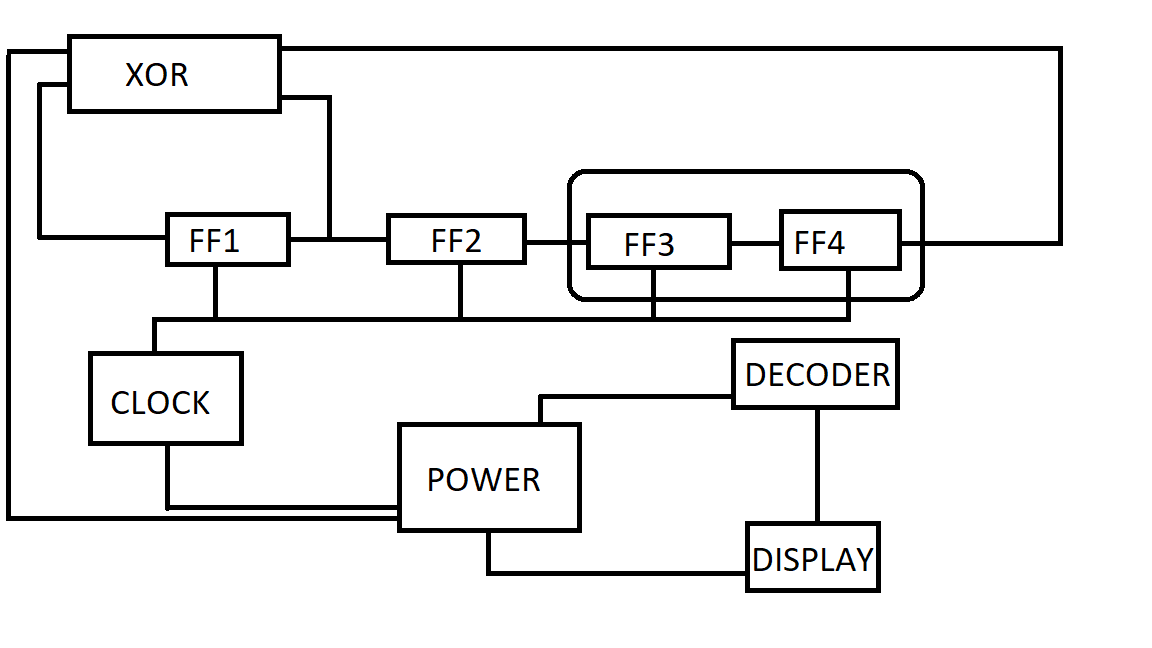
\includegraphics[width=\linewidth]{figs/diagram.png}
    \caption{Block diagram}
    \label{fig:my_label}
\end{figure}


We obtained different digits which was continuously flickering on the seven segment display the output is shown in figure 
\begin{figure}
    \centering
    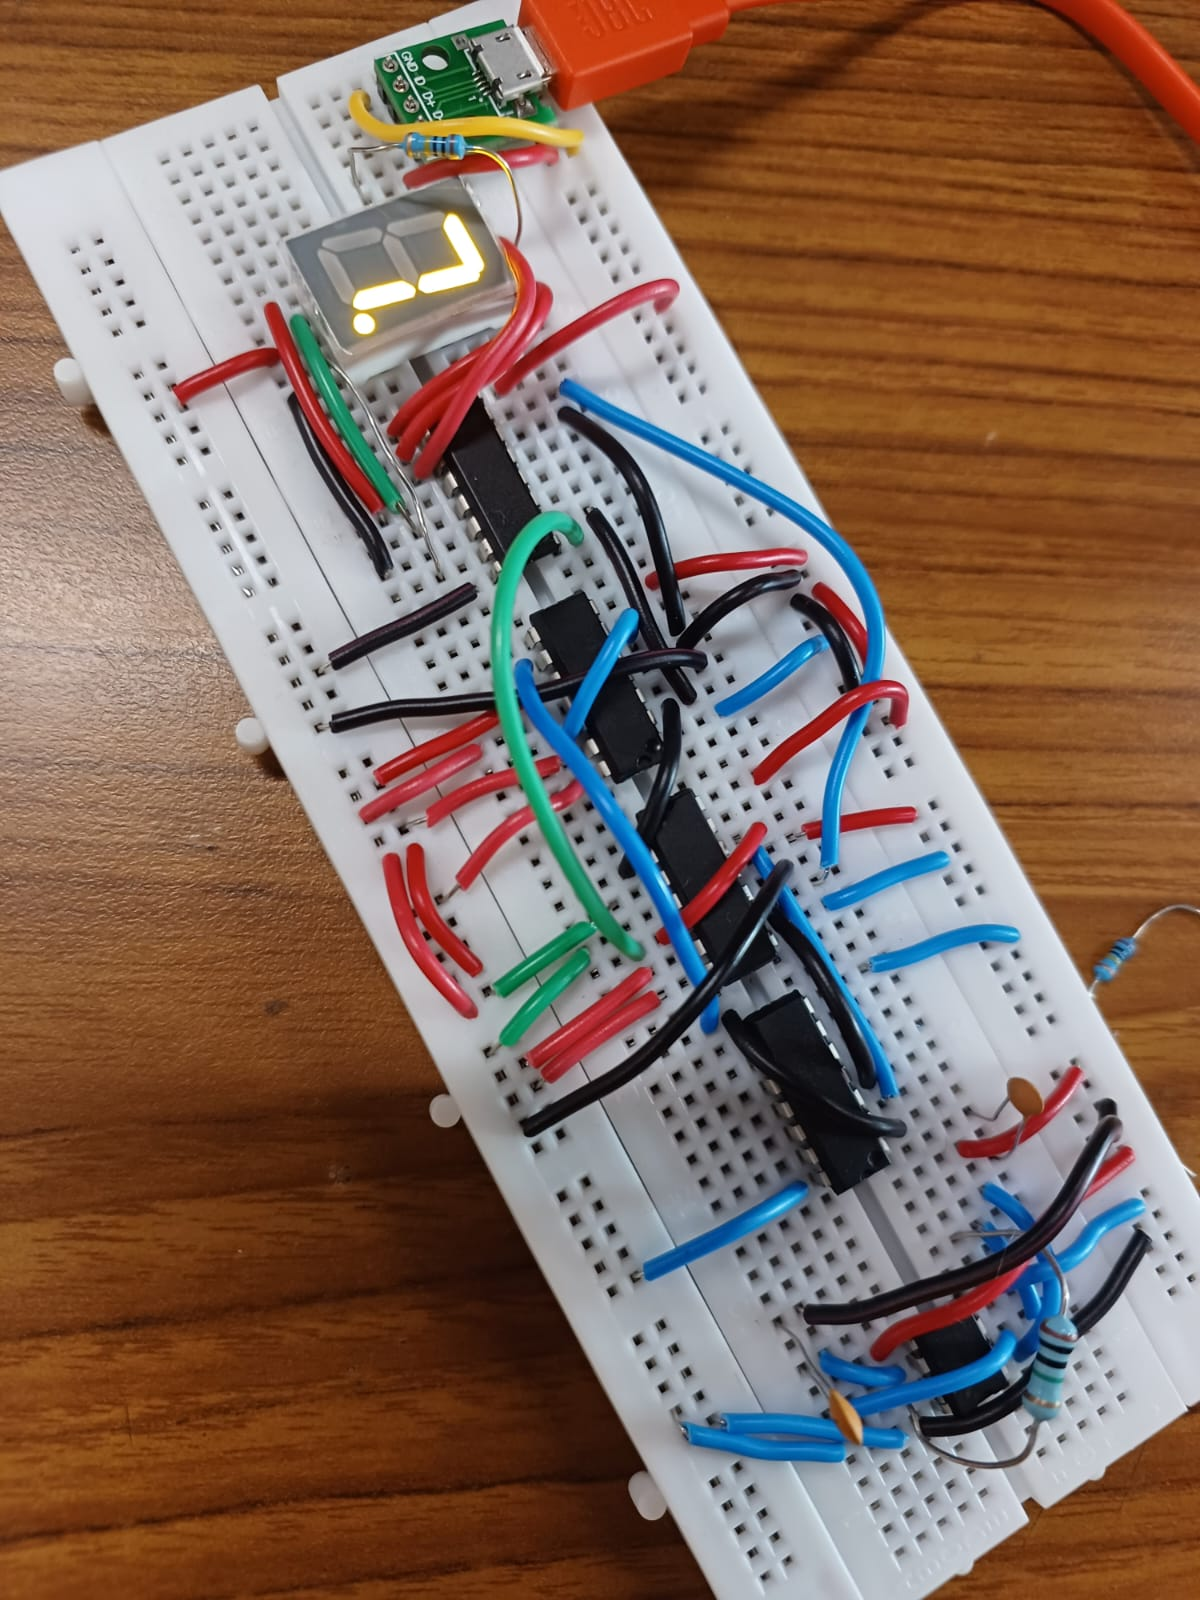
\includegraphics[width=\linewidth]{figs/clock.jpeg}
    \caption{Caption}
    \label{fig:my_label}
\end{figure}

\section{}

\end{document}


